\documentclass[12pt]{article}
\usepackage[a4paper, margin=2cm, top=1.5cm]{geometry}

\usepackage[backend=biber]{biblatex}
\addbibresource{../../references/references.bib}

\usepackage{graphicx}
\usepackage{tikz}
\usepackage{pgfplots}
\usepackage{pgfplotstable}

\usetikzlibrary{decorations.markings}
\usetikzlibrary{arrows.meta,pgfplots.units}
\usetikzlibrary{plotmarks,angles}
\usetikzlibrary{math}
\usepgfplotslibrary{colorbrewer}
\usepgfplotslibrary{fillbetween}
\pgfplotsset{width=12cm}
\pgfplotsset{compat=1.18}

\usepackage{titling}
\usepackage[separate-uncertainty=true,multi-part-units=single]{siunitx}
\usepackage{amsmath, amssymb}
\usepackage{physics}
\usepackage{circuitikz}
\usepackage{makecell}
\usepackage{booktabs}
\usepackage{scalerel}
\usepackage{float}
\usepackage{multicol}
\usepackage{multirow}
\usepackage{titling}
\usepackage{subcaption}
\usepackage{bm}
\usepackage{nicefrac}
\usepackage{diagbox}
\usepackage{minted}
\usepackage{pdfpages}
\usepackage[shortlabels]{enumitem}
\usepackage{mathtools}


\AtBeginDocument{\RenewCommandCopy\qty\SI}

\setlength{\droptitle}{-5em}

\title{Aircraft Wing Analysis Report}
\author{Luka Pivovarsky}
\date{June 2026}


\begin{document}

\maketitle

\section{Introduction}
\section{Model Validity}
\subsection{Panel Count}
\subsection{NACA Foil Comparison}
\subsection{Viscous Coupling}
The assumption that a boundary layer always remains much thinner than the section under study is not always valid - by the trailing edge of an airfoil, at low Reynolds numbers, the displacement thickness can be on the order of \qty{1}{\percent} of the chord, which is of similar order to 
\subsection{Transition Modelling}
The natural transition model used is not physically based, but instead empirical. Given that the turbulent portion of the boundary layer, in general, contributes substantially more than the laminar section to the profile drag, accurately assessing the transition point is very important for drag prediction accuracy. A more accurate method would be to use a form of the $e^n$ model, which considers the boundary layer to have transitioned when the present Tollmien-Schilling waves reach a disturbance amplification factor of $e^{n_\mathrm{crit}}$, where $n_\mathrm{crit}$ is user-set and dependent on the expected conditions of the incoming freestream flow (a more turbulent freestream will have larger disturbances that could be amplified to cause transition, and so require a lower $n_\mathrm{crit}$; for an undisturbed flow, $n_\mathrm{crit} \approx 11$, for a typical wind tunnel flow $n_\mathrm{crit} \approx 9$) \cite{boundarylayersyoung}. 
\subsection{Laminar Separation Bubbles}
Our current treatment of laminar separation bubbles considers them to be no different to attached turbulent flow. This is a dubious assumption, especially given the importance of laminar separation bubble contributions to drag on a mostly laminar airfoil \cite{lowspeeddesign}. This necessitates accurate modelling in order to give good results at low speeds.
\subsection{Turbulent Separation}
Due to the lack of inviscid to viscous coupling, the modelling of turbulent separation is fundamentally inaccurate, as there is no impact on the inviscid lift coefficient, meaning that the stall behaviour seen in real airfoils is completely absent. 

This effect also accounts for the abscence of very strong adverse pressure gradient near the trailing edge, as the finite thickness of the wake means that the outer flow does not stagnate, as it does not come to a sharp point. This particular effect is handled explicitly by the model, but there is no further.
\subsection{NACA Airfoil Comparison}
Airfoil experimental taken is due to Abbott and von Doenhoff \cite{theoryofwingsections}.
\begin{figure}[H]
    \centering
    \begin{minipage}{8cm}
        \centering
        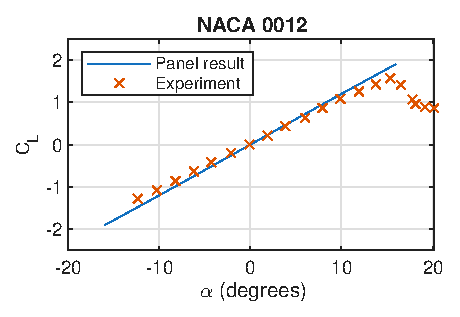
\includegraphics[width=\linewidth]{../../Figures/naca0012_clalpha.eps}
    \end{minipage}
    \hfill
    \begin{minipage}{8cm}
        \centering
        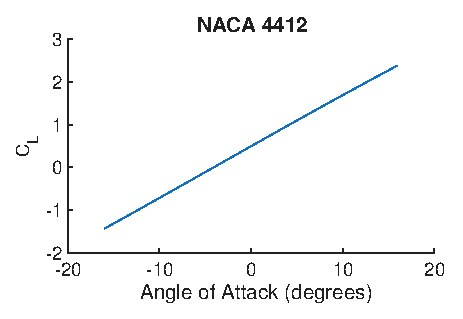
\includegraphics[width=\linewidth]{../../Figures/naca4412_clalpha.eps}
    \end{minipage}
    \caption{$C_L - \alpha$ curves}
    \label{fig:cl alpha}
\end{figure}
\begin{figure}[H]
    \centering
    \begin{minipage}{8cm}
        \centering
        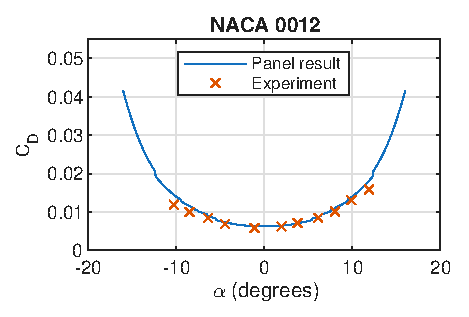
\includegraphics[width=\linewidth]{../../Figures/naca0012_cdalpha.eps}
    \end{minipage}
    \hfill
    \begin{minipage}{8cm}
        \centering
        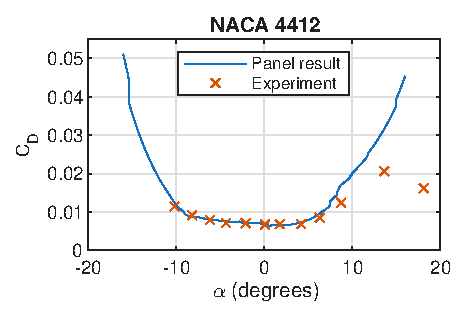
\includegraphics[width=\linewidth]{../../Figures/naca4412_cdalpha.eps}
    \end{minipage}
        \caption{$C_D - \alpha$ curves}
    \label{fig:cd alpha}
\end{figure}

\begin{figure}[H]
    \centering
    \begin{minipage}{8cm}
        \centering
        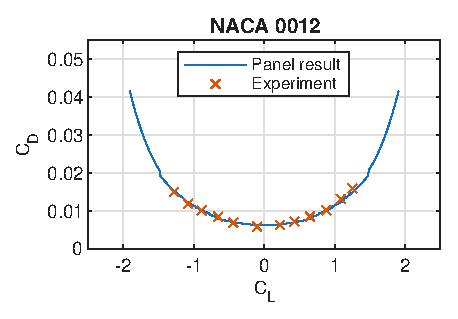
\includegraphics[width=\linewidth]{../../Figures/naca0012_clcd.eps}
    \end{minipage}
    \hfill
    \begin{minipage}{8cm}
        \centering
        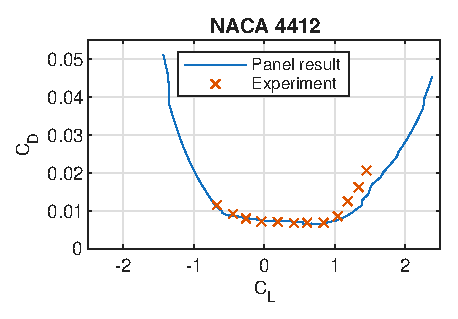
\includegraphics[width=\linewidth]{../../Figures/naca4412_clcd.eps}
    \end{minipage}
        \caption{$C_D - C_L$ curves}
    \label{fig:cl cd}
\end{figure}
\subsubsection{$C_L - \alpha$}
Close to but not entirely straight over typical incidences; at higher incidences, turbulent separation starts to occur near the trailing edge, with the separation point moving forward with increasing incidence. The effect of the separation is to cause early pressure recovery on the upper surface, as shown in Fig. \ref{fig:separation_cp}.

The \qty{4}{\percent} camber of the 4412 section evidently results in trailing edge stall as the critical mode, given the gradual loss of lift observed experimentally. The uncambered 0012 section experiences a higher peak $C_L$, but a more rapid loss of lift due to ``bubble burst''. 

\begin{figure}[H]
    \centering
    % \includegraphics[width=0.5\linewidth]{}
    \caption{*** Extract from Xfoil}
    \label{fig:separation_cp}
\end{figure}
turbulent separation leads to a decrease in lift (and hence lift-curve slope), eventually leading to a peak and then decrease before total stall. Because there is no viscous-to-inviscid coupling in our panel method, the changes to the $c_p$ distribution and hence $C_L$ due to turbulent separation are not accounted for, and so no drop-off in lift is predicted.

Positive camber shifts the zero lift incidence to some negative angle; the panel method matches experiment well, as this is mostly an inviscid effect, and in fact was historically quite accurately accounted for by use of thin aerofoil theory, as in the design of the NACA 6-series \cite{naca6seriessummary}.
\subsubsection{$C_D - \alpha$}
For symmetric airfoil, trivially symmetric around 0 incidence; both experiment and code agree.

\subsubsection{$C_D - C_L$}
These compare less well with experiment than $C_D - \alpha$ plots, simply because the evaluation of $C_L$ at a given incidence is less accurate.

The 0012 values are more accurate, which follows from the more accurate $C_L$ estimations, and stall onset at a higher angle of attack.

High $C_L/C_D$ is achieved at the edge of the ``laminar bucket '', i.e. the maximum incidence before there is a drastic rise in drag. More relevant in the 4412. Camber shifts the laminar bucket in incidence, and generally allows for higher peak $C_L/C_D$ \cite{fluiddynamicdrag}.
\section{Design Process}
\subsection{Tools}
\begin{figure}[H]
    \centering
    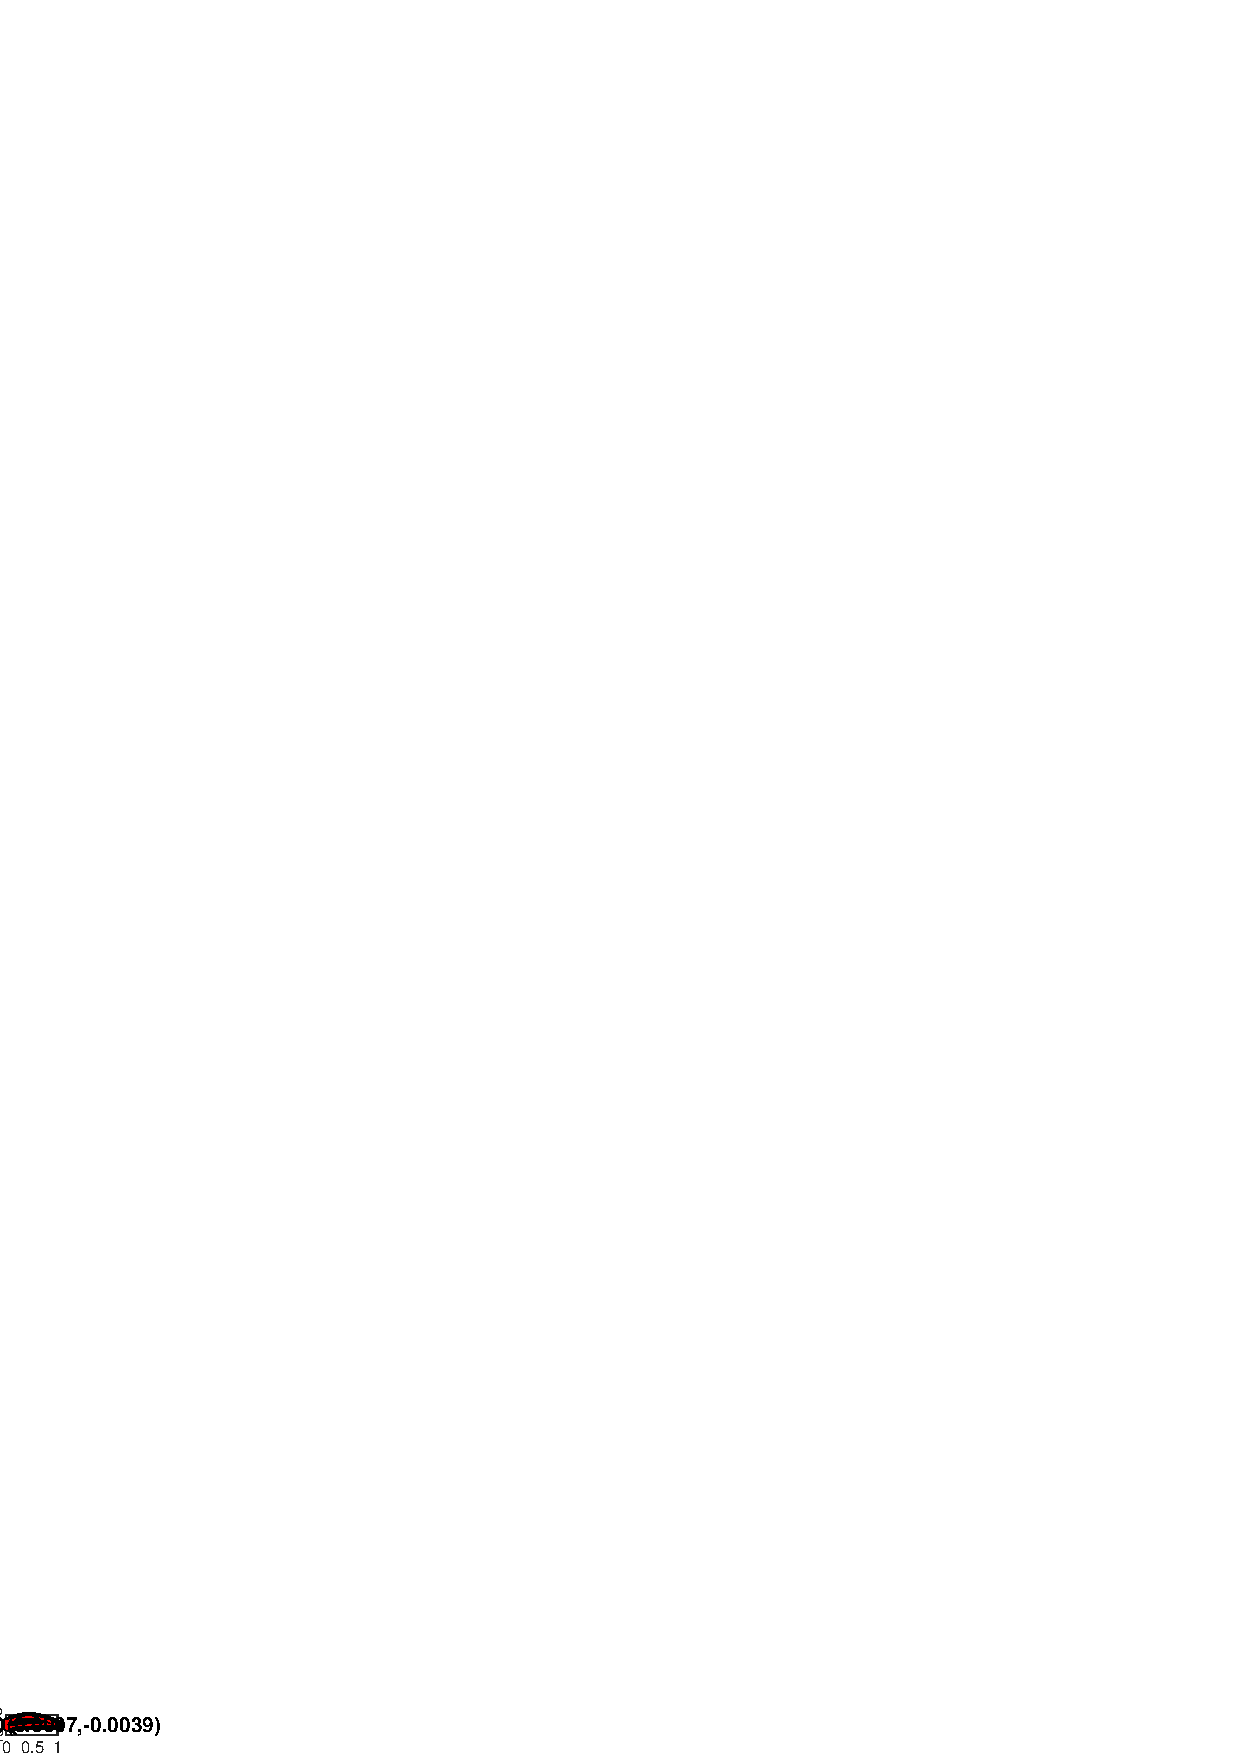
\includegraphics[width=0.95\linewidth]{../../Figures/curvature}
    \caption{Caption}
    \label{fig:placeholder}
\end{figure}
The WASG tool was modified with the ability to determine the local curvature at any point on the airfoil, shown as a curvature comb. This proved very necessary due to the sensitivity of the boundary model to very small changes in the rate of change of curvature around the airfoil. Since the cubic splines used to construct the profile are only $C^2$ continuous, explicit care had to be taken to ensure that spline-induced curvature variation did not cause premature laminar separation.

This was much more of an issue at low Reynolds numbers, as the turbulent boundary layer present at higher Reynolds numbers was much more resistant to curvature variations. This sensitivity does however indicate that the performance of the low speed laminar section would in reality be very sensitive to surface imperfections, as even very small variations caused substantial variations in $m$ and hence premature separation.
\subsection{Inverse Design}
Inverse design methods are broadly split into those based on conformal mappings of flow around a cylinder and those based on panel methods. In principle one can specify a known set of velocities (and hence $\gamma$ values) at panel edges, rather than the panel locations, and then construct a set of equations to determine the necessary edge coordinates. This problem is non-linear, unlike the forwards problem solved in our inviscid panel solver, but this can be solved effectively with Newton iteration \cite{xfoil}. This is most useful where some parts of the airfoil geometry need to be directly specified.

The conformal mapping-based methods are generally easier to use when such constraints are not present. The basic conformal mapping formulation due originally to Lighthill \cite{lighthill} and refined by Eppler and Somers \cite{epplerandsomers} is widely implemented (by Xfoil, PROFOIL, and by our own implementation in MATLAB). It is outlined below.

A conformal mapping method can either vary the shape of the (slightly perturbed) cylinder (in the manner of Theodorsen, though this is not an inverse method ***, or the Joukowsky airfoils), or the conformal mapping function itself can be altered, subject to certain constraints in order to produce a closed airfoil. 
\section{Optimisation}
\subsection{Low Speed}
At a Reynolds number as low as \num{5e5}, it is possible to retain laminar flow over a substantial fraction of the airfoil. In order to take advantage of the slow growth of the laminar boundary layer, it is desirable to delay the presence of any adverse pressure gradients that might destabilise the laminar boundary layer to as far to the rear of the airfoil as possible.

Since there is no substantial downside of a strong favourable pressure gradient, and, for a given amount of drag, we should want the lowest $c_p$ value achievable over the widest possible range of positions on the upper surface of the airfoil, it is desirable to reach the minimum $c_p$ very close to the nose of the airfoil, then remain at constant $c_p$ for a substantial fraction of the chord length, and then, to reach the trailing edge with minimum instantaneous adverse pressure gradient magnitude, by linear increase in $c_p$. Between these two sections, there is a ``transition ramp'' where the two are joined smoothly; for low Reynolds numbers the properties of this ramp can have a significant impact, as they determine whether transition will occur naturally or by laminar separation with turbulent reattachment. This is similar reasoning to that used to produce the NACA 6- and 7-series airfoils \cite{naca6seriessummary}, and many other modern laminar airfoils.
\subsection{NACA0012}
Starting point. Max L/D is 58.826 at 7.6 deg at Cl = 0.9145
\begin{figure}[H]
    \centering
    \begin{minipage}{0.49\textwidth}
        \centering
        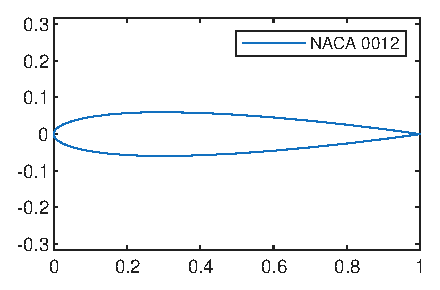
\includegraphics[width=\linewidth]{../../Figures/NACA0012.eps}
    \end{minipage}
    \hfill
    \begin{minipage}{0.49\textwidth}
        \centering
        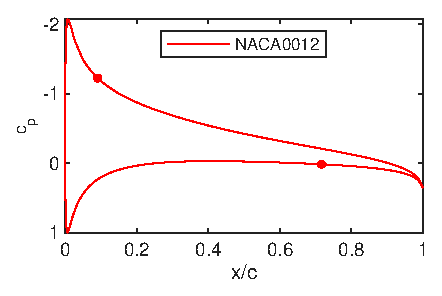
\includegraphics[width=\linewidth]{../../Figures/cp_NACA0012}
    \end{minipage}
    \caption{Airfoil shape and $c_p$ plot ($\alpha=5^{\circ}$) for NACA0012.}
    \label{fig:NACA0012_1}
\end{figure}

    \begin{figure}[H]
    \centering
    \begin{minipage}{0.49\textwidth}
        \centering
        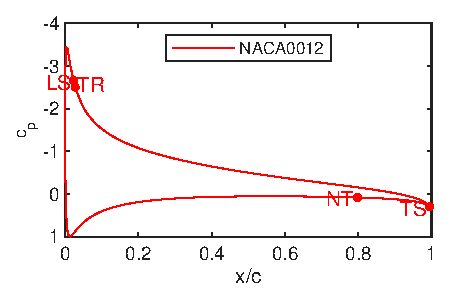
\includegraphics[width=\linewidth]{../../Figures/cp_NACA0012_7deg.eps}
    \end{minipage}
    \hfill
    \begin{minipage}{0.49\textwidth}
        \centering
        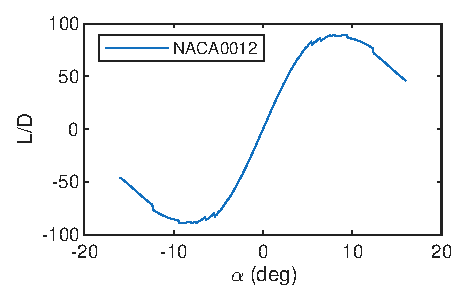
\includegraphics[width=\linewidth]{../../Figures/ld_NACA0012.eps}
    \end{minipage}
        \caption{$c_p$ plot ($\alpha=7^{\circ}$) and \(L/D\) curves for NACA0012.}
    \label{fig:NACA0012_2}
\end{figure}
\subsubsection{LLL01}

The airfoil thickness was increased to 15\% to reduce the severity of the suction peak, creating a NACA 0015 equivalent airfoil: LLL01. This has a slightly lower maximum lift-to-drag ratio than the NACA 0012: 53.3 at $\alpha=4.9^{\circ}$ ($C_L = 0.605$).

\begin{figure}[H]
    \centering
    \begin{minipage}{0.49\textwidth}
        \centering
        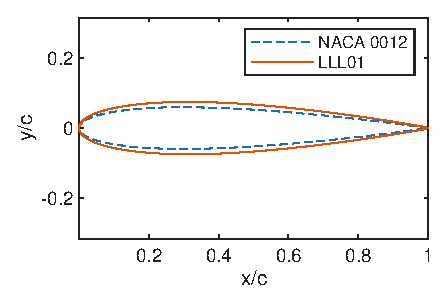
\includegraphics[width=\linewidth]{../../Figures/LLL01.eps}
    \end{minipage}
    \hfill
    \begin{minipage}{0.49\textwidth}
        \centering
        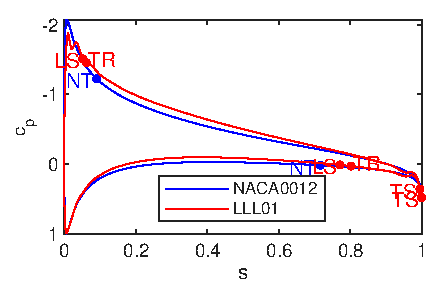
\includegraphics[width=\linewidth]{../../Figures/cp_LLL01}
    \end{minipage}
    \caption{Airfoil shape and $c_p$ plot ($\alpha=5^{\circ}$) for LLL01.}
    \label{fig:LLL01_1}
        \end{figure}

Although the adverse pressure gradient after the suction peak is slightly reduced, this is not sufficient to delay separation and turbulent transition.

    
    \begin{figure}[H]
    \centering
    \begin{minipage}{0.49\textwidth}
        \centering
        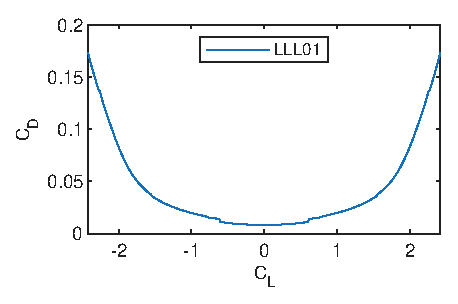
\includegraphics[width=\linewidth]{../../Figures/cdcl_LLL01.eps}
    \end{minipage}
    \hfill
    \begin{minipage}{0.49\textwidth}
        \centering
        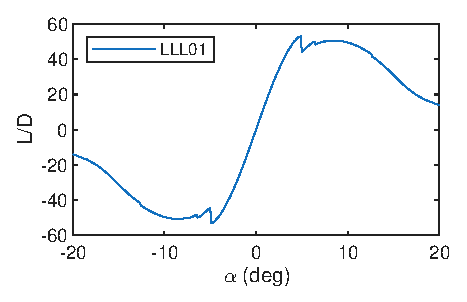
\includegraphics[width=\linewidth]{../../Figures/ld_LLL01.eps}
    \end{minipage}
        \caption{$C_D-C_L$ and \(L/D\) curves for LLL01.}
    \label{fig:LLL01_2}
\end{figure}

There is now a visible `laminar bucket' region on the $C_D- C_L$ curve, centred at zero incidence. This suggests that the lift-to-drag ratio may improve if the zero incidence $C_L$ were increased: by adding camber.

\subsubsection{LLL02}

2\% camber was added to LLL01 with a maximum at 40\% chord, increasing \(L/D\) to a maximum of 78.8 at $\alpha=6.1^{\circ}$ $(C_L = 1.005)$.

\begin{figure}[H]
    \centering
    \begin{minipage}{0.49\textwidth}
        \centering
        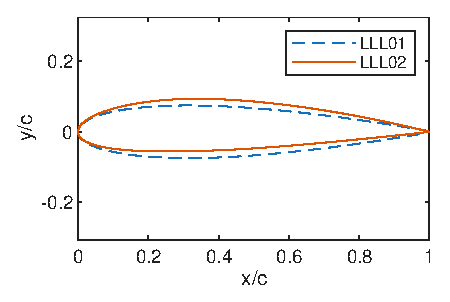
\includegraphics[width=\linewidth]{../../Figures/LLL02.eps}
    \end{minipage}
    \hfill
    \begin{minipage}{0.49\textwidth}
        \centering
        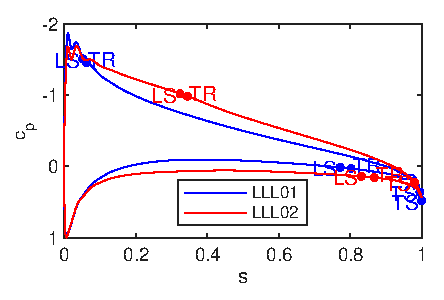
\includegraphics[width=\linewidth]{../../Figures/cp_LLL02}
    \end{minipage}
    \caption{Airfoil shape and $c_p$ plot ($\alpha=5^{\circ}$) for LLL02.}
    \label{fig:LLL02_1}
        \end{figure}

    Laminar separation is delayed on both upper and lower surfaces due to the gentler adverse pressure gradient.
    
    \begin{figure}[H]
    \centering
    \begin{minipage}{0.49\textwidth}
        \centering
        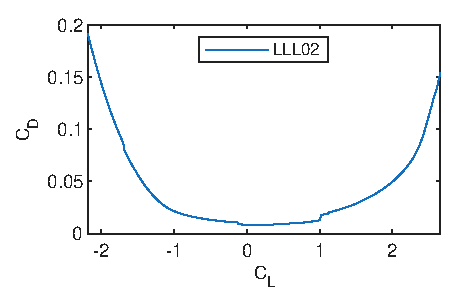
\includegraphics[width=\linewidth]{../../Figures/cdcl_LLL02.eps}
    \end{minipage}
    \hfill
    \begin{minipage}{0.49\textwidth}
        \centering
        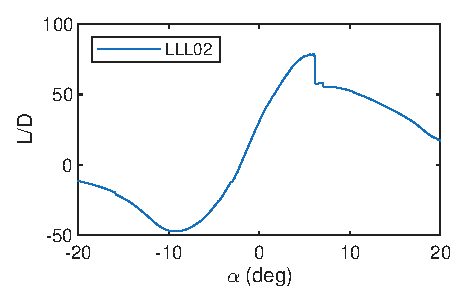
\includegraphics[width=\linewidth]{../../Figures/ld_LLL02.eps}
    \end{minipage}
        \caption{$C_D-C_L$ and \(L/D\) curves for LLL02.}
    \label{fig:LLL02_2}
\end{figure}

As predicted, the `laminar bucket' in the $C_D-C_L$ curve is shifted to positive $C_L$. Gains in \(L/D\) ratio are made due to the camber-derived lift increase, and the delay in laminar separation on the upper and lower surfaces. 

The sharp drop in \(L/D\) occurs after $\alpha=6.1^{\circ}$, where the laminar separation point abruptly moves upstream toward the leading edge. In the region downstream of the suction peak, the Thwaites parameter $m$ oscillates, approaching the separation threshold of 0.09 repeatedly without crossing it. Consequently, a sudden jump in separation location can occur when any oscillation overshoots the critical value.

\subsubsection{LLL03}

To further reduce the post suction peak adverse pressure gradient, the maximum thickness point was moved rearward to 35\% chord. The maximum \(L/D\) increases to 84.3 at $\alpha=6^{\circ}$ ($C_L=0.996$).

\begin{figure}[H]
    \centering
    \begin{minipage}{0.49\textwidth}
        \centering
        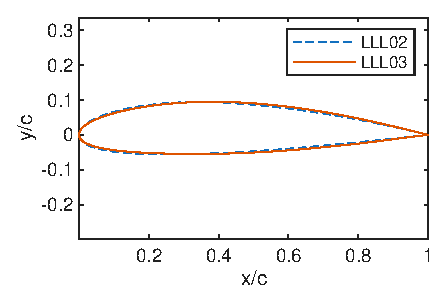
\includegraphics[width=\linewidth]{../../Figures/LLL03.eps}
    \end{minipage}
    \hfill
    \begin{minipage}{0.49\textwidth}
        \centering
        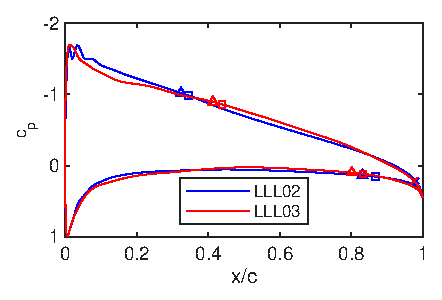
\includegraphics[width=\linewidth]{../../Figures/cp_LLL03}
    \end{minipage}
    \caption{Airfoil shape and $c_p$ plot ($\alpha=5^{\circ}$) for LLL03.}
    \label{fig:LLL03_1}
        \end{figure}

    The desired laminar separation delay is achieved, and the maximum \(L/D\) rises accordingly.
    
    \begin{figure}[H]
    \centering
    \begin{minipage}{0.49\textwidth}
        \centering
        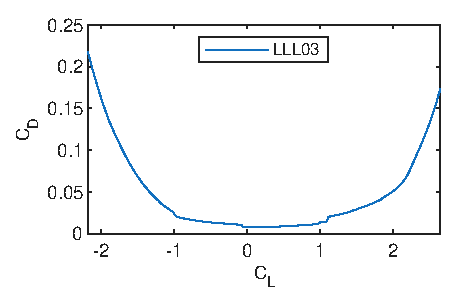
\includegraphics[width=\linewidth]{../../Figures/cdcl_LLL03.eps}
    \end{minipage}
    \hfill
    \begin{minipage}{0.49\textwidth}
        \centering
        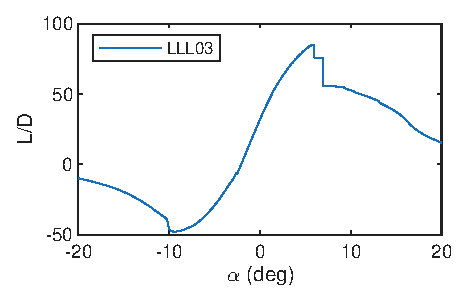
\includegraphics[width=\linewidth]{../../Figures/ld_LLL03.eps}
    \end{minipage}
        \caption{$C_D-C_L$ and \(L/D\) curves for LLL03.}
    \label{fig:LLL03_2}
\end{figure}

Similar to LLL02, the sharp \(L/D\) drops result from oscillations in $m$, however here the separation advances in multiple, smaller steps.



\subsubsection{LLL04}

The next progression was to increase the camber to 4\%, with the maximum point at 50\% (from 40\%). The thickness has remained unchanged throughout at 15\% with a maximum at 35\% chord. Further improvements are made, with a new maximum \(L/D\) of 91.4 at $\alpha=5.6^{\circ}$ ($C_L=1.26$).

\begin{figure}[H]
    \centering
    \begin{minipage}{0.49\textwidth}
        \centering
        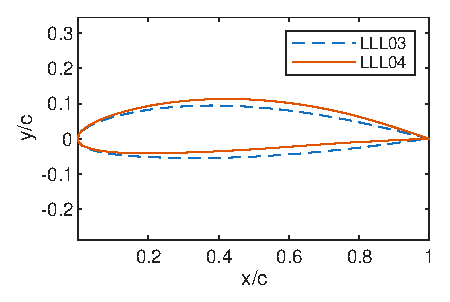
\includegraphics[width=\linewidth]{../../Figures/LLL04.eps}
    \end{minipage}
    \hfill
    \begin{minipage}{0.49\textwidth}
        \centering
        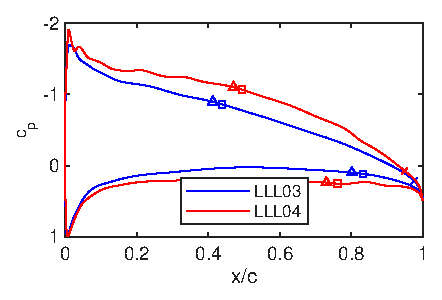
\includegraphics[width=\linewidth]{../../Figures/cp_LLL04}
    \end{minipage}
    \caption{Airfoil shape and $c_p$ plot ($\alpha=5^{\circ}$) for LLL04.}
    \label{fig:LLL04_1}
        \end{figure}

    Improvements mainly result from the increase in lift, however the upper laminar separation point has also moved rearward, due to the gentler adverse pressure gradient. The pressure distribution on the lower surface is also becoming flatter.
    
    \begin{figure}[H]
    \centering
    \begin{minipage}{0.49\textwidth}
        \centering
        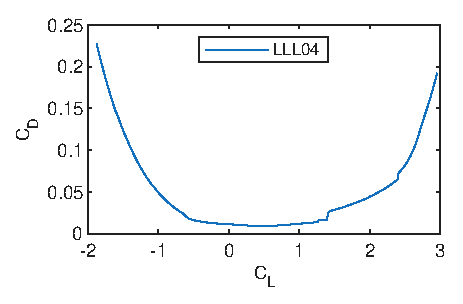
\includegraphics[width=\linewidth]{../../Figures/cdcl_LLL04.eps}
    \end{minipage}
    \hfill
    \begin{minipage}{0.49\textwidth}
        \centering
        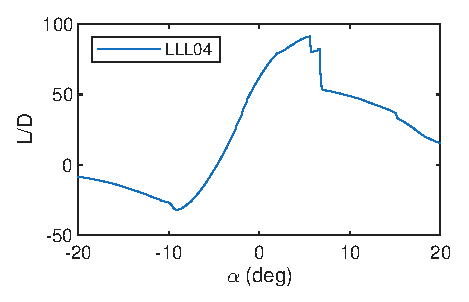
\includegraphics[width=\linewidth]{../../Figures/ld_LLL04.eps}
    \end{minipage}
        \caption{$C_D-C_L$ and \(L/D\) curves for LLL04.}
    \label{fig:LLL04_2}
\end{figure}

\subsubsection{LLL05}

Further \(L/D\) improvements are reached by increasing camber to  7\%, with a maximum at 50\% chord. Maximum \(L/D\) is now 100.4 at $\alpha=2.3^{\circ}$ ($C_L = 1.28$).

\begin{figure}[H]
    \centering
    \begin{minipage}{0.49\textwidth}
        \centering
        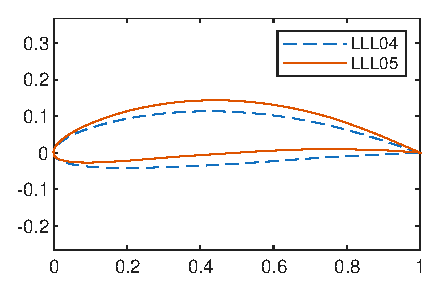
\includegraphics[width=\linewidth]{../../Figures/LLL05.eps}
    \end{minipage}
    \hfill
    \begin{minipage}{0.49\textwidth}
        \centering
        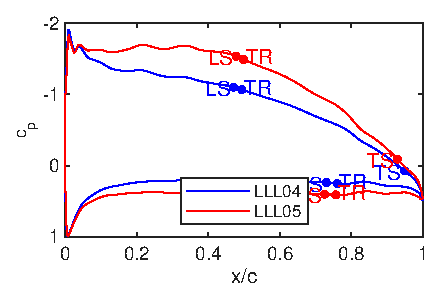
\includegraphics[width=\linewidth]{../../Figures/cp_LLL05}
    \end{minipage}
    \caption{Airfoil shape and $c_p$ plot ($\alpha=5^{\circ}$) for LLL05.}
    \label{fig:LLL05_1}
        \end{figure}

    As for LLL04, the improvements observed are mainly due to the increase in lift, as the separation locations and trailing‑edge momentum thicknesses are virtually unchanged. However, the $c_p$ distribution has desirably flattened out.
    
    \begin{figure}[H]
    \centering
    \begin{minipage}{0.49\textwidth}
        \centering
        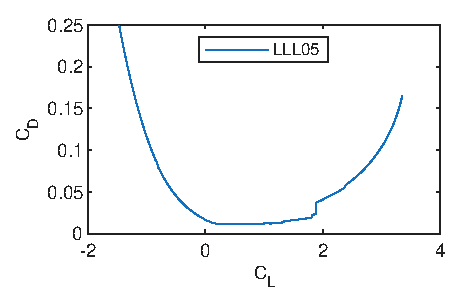
\includegraphics[width=\linewidth]{../../Figures/cdcl_LLL05.eps}
    \end{minipage}
    \hfill
    \begin{minipage}{0.49\textwidth}
        \centering
        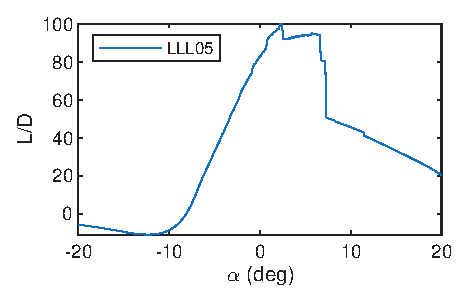
\includegraphics[width=\linewidth]{../../Figures/ld_LLL05.eps}
    \end{minipage}
        \caption{$C_D-C_L$ and \(L/D\) curves for LLL05.}
    \label{fig:LLL05_2}
\end{figure}

% \subsubsection{LLL06} ** Could possibly remove this and consolidate **

% At this stage, manual geometry manipulation was performed using the \texttt{wasg} tool, moving beyond simple camber and thickness adjustments. Following the modifications described in Section~\ref{sec:wasg}, the leading‑edge curvature became smoother due to the reduction in the number of spline knots, as evident in the $c_p$ plot.

% \begin{figure}[H]
%     \centering
%     \begin{minipage}{0.49\textwidth}
%         \centering
%         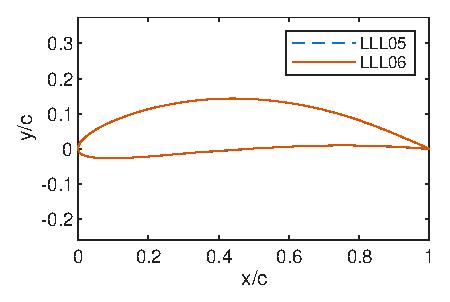
\includegraphics[width=\linewidth]{../../Figures/LLL06.eps}
%     \end{minipage}
%     \hfill
%     \begin{minipage}{0.49\textwidth}
%         \centering
%         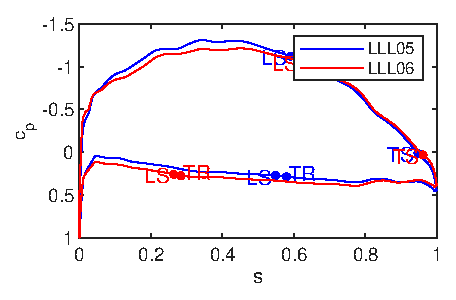
\includegraphics[width=\linewidth]{../../Figures/cp_LLL06}
%     \end{minipage}
%     \caption{Airfoil shape and $c_p$ plot ($\alpha=5^{\circ}$) for LLL06.}
%     \label{fig:LLL06_1}
%         \end{figure}

% The geometry changes (Fig.~\ref{fig:LLL06_1}) were subtle, focusing on smoothing the lower‑surface curvature. Laminar separation was delayed, however \(L/D\) only reached 101.3 at $\alpha=2.9^{\circ}$ ($C_L = 1.34$). The small gain may be because the lower surface contributes much less to the momentum thickness than the upper surface; further improvement would requires upper surface modifications.
    
    \begin{figure}[H]
    \centering
    \begin{minipage}{0.49\textwidth}
        \centering
        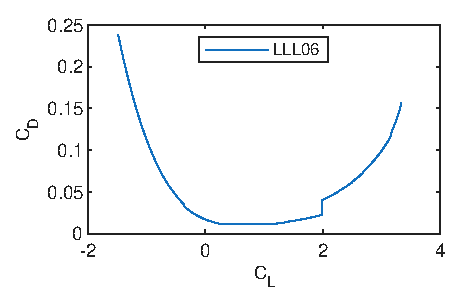
\includegraphics[width=\linewidth]{../../Figures/cdcl_LLL06.eps}
    \end{minipage}
    \hfill
    \begin{minipage}{0.49\textwidth}
        \centering
        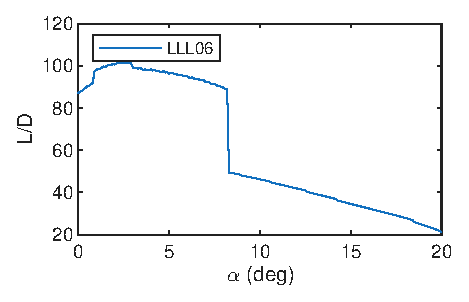
\includegraphics[width=\linewidth]{../../Figures/ld_LLL06.eps}
    \end{minipage}
        \caption{$C_D-C_L$ and \(L/D\) curves for LLL06.}
    \label{fig:LLL06_2}
\end{figure}

\subsubsection{LLL07}

For this iteration, the priority was to smooth the leading edge portion of the $c_p$ plot. This was achieved, with little difference in maximum \(L/D\): 104.3 at $\alpha=4.6^{\circ}$ ($C_L=1.57$).

\begin{figure}[H]
    \centering
    \begin{minipage}{0.49\textwidth}
        \centering
        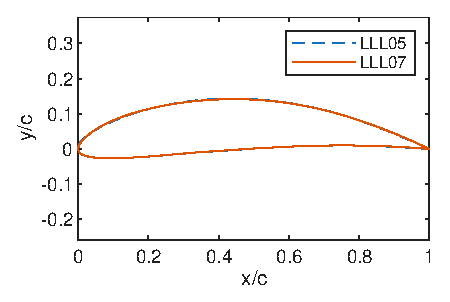
\includegraphics[width=\linewidth]{../../Figures/LLL07.eps}
    \end{minipage}
    \hfill
    \begin{minipage}{0.49\textwidth}
        \centering
        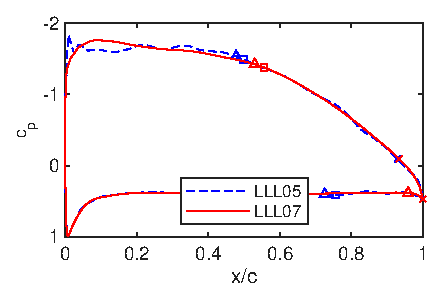
\includegraphics[width=\linewidth]{../../Figures/cp_LLL07}
    \end{minipage}
    \caption{Airfoil shape and $c_p$ plot ($\alpha=5^{\circ}$) for LLL07.}
    \label{fig:LLL07_1}
        \end{figure}

    
    \begin{figure}[H]
    \centering
    \begin{minipage}{0.49\textwidth}
        \centering
        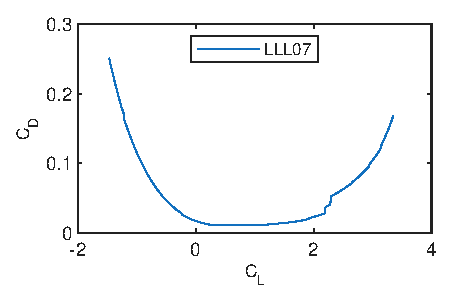
\includegraphics[width=\linewidth]{../../Figures/cdcl_LLL07.eps}
    \end{minipage}
    \hfill
    \begin{minipage}{0.49\textwidth}
        \centering
        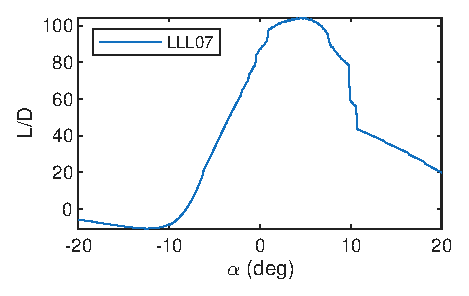
\includegraphics[width=\linewidth]{../../Figures/ld_LLL07.eps}
    \end{minipage}
        \caption{$C_D-C_L$ and \(L/D\) curves for LLL07.}
    \label{fig:LLL07_2}
\end{figure}

The small gain in \(L/D\) is attributed to a slight delay in upper surface laminar separation. Curvature smoothing has also reduced oscillations in the Thwaites parameter $m$, resulting in a smoother \(L/D\) curve. Consequently, LLL07 has a more stable operating point than LLL04, with fewer sudden efficiency drops.

\subsubsection{LLL08}

After modifying the upper trailing‑edge geometry, natural transition was achieved at the maximum \(L/D\) operating point. However, turbulent separation began earlier than LLL07, limiting \(L/D\) to 112.7 at \(\alpha = 3.1^\circ\) (\(C_L = 1.39\)). A sudden drop in \(L/D\) occurs at \(\alpha = 3.1^\circ\), where a laminar separation bubble reappears. This illustrates that often increasing \(L/D\) reduces the stable operating range. 

\begin{figure}[H]
    \centering
    \begin{minipage}{0.49\textwidth}
        \centering
        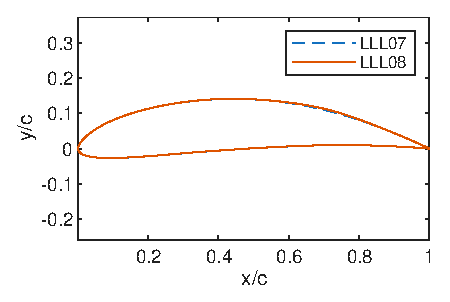
\includegraphics[width=\linewidth]{../../Figures/LLL08.eps}
    \end{minipage}
    \hfill
    \begin{minipage}{0.49\textwidth}
        \centering
        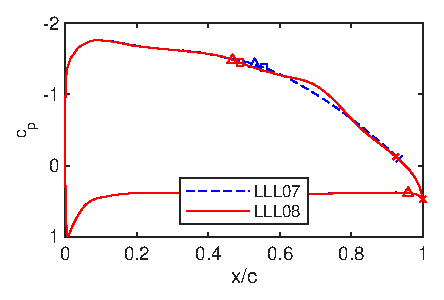
\includegraphics[width=\linewidth]{../../Figures/cp_LLL08}
    \end{minipage}
    \caption{Airfoil shape and $c_p$ plot ($\alpha=5^{\circ}$) for LLL08.}
    \label{fig:LLL08_1}
        \end{figure}
    
    \begin{figure}[H]
    \centering
    \begin{minipage}{0.49\textwidth}
        \centering
        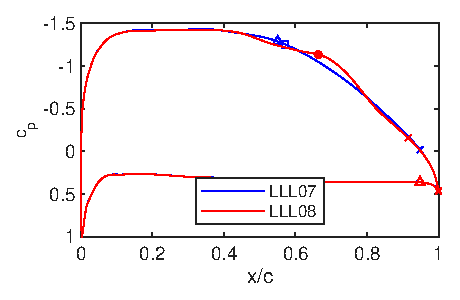
\includegraphics[width=\linewidth]{../../Figures/cp_LLL08_3deg.eps}
    \end{minipage}
    \hfill
    \begin{minipage}{0.49\textwidth}
        \centering
        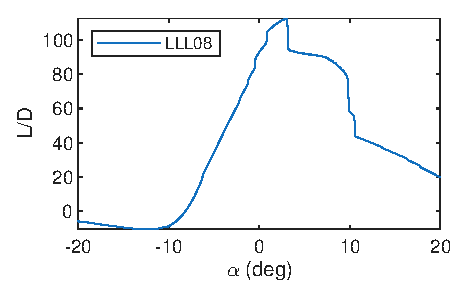
\includegraphics[width=\linewidth]{../../Figures/ld_LLL08.eps}
    \end{minipage}
        \caption{$c_p$ plot ($\alpha=3^{\circ}$) and \(L/D\) curves for LLL08.}
    \label{fig:LLL08_2}
\end{figure}

Beyond this point, manual improvements could not be made using \texttt{wasg}; small changes in curvature caused early laminar or turbulent separation. Ideally, turbulent separation would not occur before the trailing edge on either surface, however this was difficult to implement manually.
\subsection{High Speed First Attempt}
Start from NACA4412
134 at 5.7
\subsubsection{LLH01}
Want to reduce suction peak to slightly delay transition (increase width of peak by increase LE radius by factor of 2, interpolating over first 10\%).

136.7 at 6.8
\subsubsection{LLH02}
Angle of attack kind of unreasonable; would prefer smaller design angle of attack, so increase camber to 7\%. Conveniently also removes much of the suction peak, delaying separation, although the maximum is limited by the slight peak that remains.

This has made the bottom worse though.
137.8 at 3.6.
\subsubsection{LLH03}
Tweak curve near nose to avoid peak entirely - increases lift somewhat and so shifts best L/D to 139 at 1.7.

\subsection{High Speed Final}
Start with 4412
\subsubsection{LLH01\_b}
Want to reduce suction peak to slightly delay transition (increase width of peak by increase LE radius by factor of 2, interpolating over first 10\%).

Messed around with interpolation region, then tried adding camber and curve tweaks. The bottom just did not benefit at all from the large curvature.

\subsubsection{LLH01\_e or possibly f}
Decerase upper surface curvature only, keeping bottom more or less the same.
145.6 at \qty{6.8}{\degree}.

\subsubsection{LLH02\_e}
(Intermediate is available if this isn't long enough).
About 80\% of the boundary layer growth is in the final 10\% of the airfoil. There's basically no amount of lift that can be coming from here to warrant the adverse pressure gradient.

Hence, the curvature of the rear half of the upper surface was reduced, with even some slight reflex added. Minor modifications to the lower surface formed a compatible trailing edge. This did result in a slightly steeper adverse pressure gradient overall, but the turbulent boundary layer was more resistant to this than a shorter very intense section.

Max L/D 152.1 at 6.9 degrees
\subsubsection{LLH04\_e\_low}
The clearest avenue for further improvement is increase the pressure on the lower surface, by adding concave curvature to the pressure surface. Most easily done by adjusting only the camber line - tried increasing camber from 4.5 up to 6.5 (with intermediates that weren't as good).
\subsubsection{LLH05\_e and Inverse}
Tried tweaking pressure surface to avoid the adverse pressure gradient that causes early transition at incidences just below peak L/D. Not really possible to make smooth enough with the direct editing tools available, so do inverse design ***.

\section{Optimal Sections}
\section{Physical Processes}
\section{Result Reliability}
Not

\printbibliography

\end{document}
